%=====================================================================
\section{Iteración 2: vuelta al modelado}

CRISP-ML(Q) no es lineal: si la evaluación no alcanza el criterio, se vuelve a la preparación de datos o al modelado. Antes de correr nada se fijó un protocolo con el candidato, la regla de selección y la regla de adopción. El diagnóstico usa solo la validación y la exploración:
\begin{itemize}
\item la deriva de las covariables (más \texttt{Reviewed-by} y más correcciones con el tiempo) sugiere entrenar con una ventana deslizante de 3 años;
\item el difuso ve 10 de las 22 variables que usan las referencias, lo que sugiere un conjunto ampliado de 19.
\end{itemize}
El diseño es un factorial $2\times 2$ evaluado en validación. Cuando cambia la ventana, el \emph{gradient boosting} se reentrena con esa misma ventana.

Una regla de adopción evita usar la prueba otra vez sin necesidad: la iteración 2 solo se evaluaría en 2026 si su razón AUC-PR$_{FE}$/AUC-PR$_{GB}$ en validación superara la de la iteración 1 (\cifItDosUmbral{}).

\textbf{Resultado} (Fig.~\ref{fig:it2}): ningún candidato la supera.
\begin{itemize}
\item ventana creciente con 10 variables (la iteración 1): \cifItDosCreOriRazon{};
\item ventana deslizante con 10 variables: \cifItDosDesOriRazon{};
\item ventana creciente con 19 variables: \cifItDosCreAmpRazon{};
\item ventana deslizante con 19 variables: \cifItDosDesAmpRazon{}.
\end{itemize}
Más variables no ayudan: el AG sigue eligiendo 3 o 4 reglas de tamaño y difusión. Una ventana más corta tampoco cambia nada, y el \emph{gradient boosting} queda igual con ella.

La iteración 2 no se adoptó y la prueba no se volvió a usar. Las cifras de la Sección~V son las definitivas.

\begin{figure}[!t]
\centering
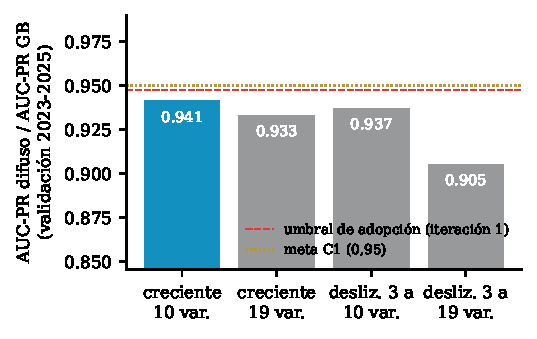
\includegraphics[width=0.88\columnwidth]{../../resultados/figuras/iteracion2_candidatos.pdf}
\caption{Iteración 2: razón de AUC-PR difuso/\emph{gradient boosting} en validación para los cuatro candidatos (semilla 11), frente al umbral de adopción.}
\label{fig:it2}
\end{figure}
